\documentclass[12pt]{article}

% math typesetting
\usepackage{array, amsmath, amssymb, amsfonts}

% layout control
\usepackage[paper=a4paper,left=25mm,right=25mm,top=20mm,bottom=25mm]{geometry}
\usepackage[onehalfspacing]{setspace}
\setlength{\parskip}{.5em}
\usepackage{rotating}
\usepackage{setspace}
\usepackage{fancyhdr}
\usepackage{parallel}
\usepackage{parcolumns}

% tables, list
\usepackage{tabularx, booktabs, multicol, multirow, longtable}
\usepackage{enumitem}

% graphics stuff
\usepackage[usenames,dvipsnames]{xcolor}
\usepackage{subfig, graphicx, tikz}
\usepackage[space]{grffile} % allows us to specify directories that have spaces
\usepackage[section]{placeins} % prevents floats from moving past a \FloatBarrier or section

% bibliography
\usepackage{natbib}
\bibpunct{(}{)}{;}{a}{}{,}
\usepackage{setspace}

% font
\usepackage{times}

% misc
\usepackage{enumitem} %no space bewteen item [nosepitem]
\usepackage{boxedminipage} % floating textbox
\usepackage{animate}
\graphicspath{ {../graph/} }
\usepackage[colorlinks=true, allcolors=MidnightBlue]{hyperref}

% -------------------- title -------------------- %

\title{Why Best Practice Does Not Work in Practice?\\
        The Political Challenge of Implementation}
\author{Anh Le - IED Intern}
\date{}

\setlength{\headheight}{15pt}
\setlength{\headsep}{20pt}
\pagestyle{fancyplain}

\fancyhf{}

\lhead{\fancyplain{}{Anh Le}}
\chead{\fancyplain{}{The Political Challenge of Implementation}}
\rhead{\fancyplain{}{\today}}
\rfoot{\fancyplain{}{\thepage}}

%%%%%%%%%%%%%%%%%%%% DOCUMENT %%%%%%%%%%%%%%%%%%%%

% \doublespacing

\begin{document}

\maketitle
\begin{abstract}
blah blah blah
\end{abstract}

\section{Introduction}
\label{sec:intro}

In the latest \citet{Integrity2012a}, which ranks countries on their anti-corruption effort, an Asian country stands out remarkably. It boasts an exemplary score of 86.9 on legal framework, higher than Germany's 81.0. It has perfect anti-corruption law, which criminalizes bribery, extortion, and misuse of public assets. Better yet, the country has established a host of supporting institutions, including a national ombudsman protected by law against political interference---something that is left for citizens to desire even in the United States \citep{MinistryofLawandJustice2003}. On top of that, there is an independent agency with the legal mandate to address corruption, whose leader can only be removed by the head of a democratically elected government, based on an inquiry by the Supreme Court.

The country in question is India, a place deeply mired for years in corruption. There are yet other countries with the same puzzling mismatch between law and practice such as China and Mongolia, whose legal framework earns a score of 78 and 80, closely in the same league with Germany (81.0). This pattern extends well beyond Asia to all corners of the developing world, including Uganda (97.8) and Kenya (83.2). These developing countries all possess, on paper at least, world-class legal systems. The intensive effort by the development community to spread knowledge and tout models has certainly paid off in this regard.

But we---as committed organizations and passionate professionals-care not about laws on paper but lives on Earth. Does the experience of corruption improve accordingly? Unfortunately not, as the rate of progress remains glacially low. Even if we use an optimistic estimate of countries' improvement rate, it will take developing countries hundreds, even thousands of years, in order to catch up with the standard of today Singapore \citep{Pritchett2010}.\footnote{We can calculate the fastest improvement rate by assuming that countries have the lowest possible starting point, set to that of Somalia today} Our relentless effort to promote best practice in institutional form has led to improvement, but only in the sense that a new anti-corruption law passed with little effect is an improvement, and that development finally achieved after hundreds of years is a success.

Of course, that is not to say all forms of technical assistance and knowledge solution are not valuable. If there is a new drug or construction technology, it should not be held back outside the countries' reach. However, in governance and anti-corruption issues, the centerpiece is people, whose political interests and interactions in each country are complicated and unique. In this setting, transplanting best governance practice is not straightforward as pouring concrete or combating viruses.

And that is the short answer to why implementation often fails. This paper will provide the longer answer, explaining how reform initiatives, from both supply and demand sides, erroneously assume that the state and the citizens are monolithic entities with a single-minded interest in better governance. On the contrary, governance and corruption are, at their core, a collective action problem, caused by the fact that the benefit of bribery and patronage (for both the official and the citizen) is immediate and concentrated, whereas the cost of poor governance is dispersed and opaque. Improving governance and fighting corruption, therefore, are fundamentally about building the political will that rallies the people and reform-minded officials under the promise of change.

Keeping in mind its key message about political will as the prerequisite of reform, this paper is structured accordingly. Section \ref{sec:principalagent} analyzes the theoretical framework of current governance initiative, showing that it think of governance as a principal-agent, instead of a collective action, problem. This thinking leads to the mistaken belief that the greatest obstacle to reform is a lack of resource and design expertise, both of which institutions such as the ADB are eager to provide \citep[16]{GlobalIntegrity2012}. Section \ref{sec:collectiveaction} discusses several case studies to emphasize that reform has always been a deeply political, not bureaucratic, matter, and that its success and failure have always depended on overcoming the collective action problem. Section \ref{sec:IB} proposes the wide adoption of "Indicators and Benchmarks" as a clever strategy for the ADB to nurture the political will for reform in a sanitized, politically-neutral manner. By comparing local performances in public sectors with an immediate impact on people's welfare, this strategy rewards reform-minded officials and invigorates the public interest in the cause of good governance.

After all, only the people themselves that can, and should, do the strenuous work of shaping their countries' trajectory. We must cheer them on, but the journey towards betterment is theirs to travel.

\begin{figure}
\begin{center}
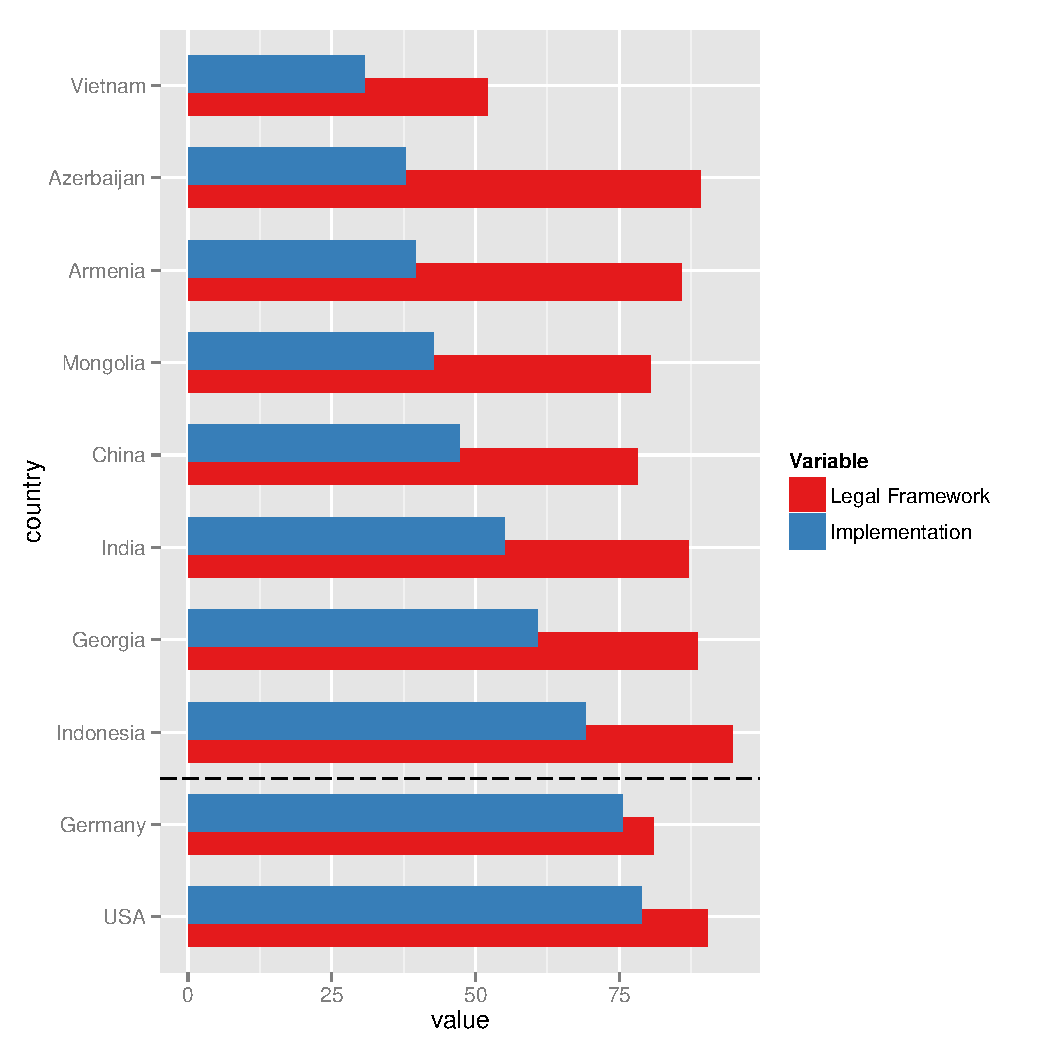
\includegraphics[scale=0.6]{implementation}
\captionof{figure}{Same legal, different implementation}
\end{center}
\end{figure}

\begin{figure}
\begin{center}
\animategraphics[autoplay,loop,controls,width=\linewidth]{1}{Rplot}{1}{13}
\captionof{figure}{The data shows that the pattern of corruption remains stubbornly stable. There is even a deteriorating trend in Asia, reflected by the darkening colors. Source: World Governance Index. Note: The animation can only be viewed in Adobe Acrobat}
\end{center}
\end{figure}

\section{The prevalent principal-agent framework}
\label{sec:principalagent}

\subsection{Supply side initiative}
\label{sec:supplyside}
Explicitly named or not, our current approach to governance and anti-corruption is deeply wedded to the principal-agent framework. In the supply side approach to governance, the principal is the government, which has the best interest of the country at heart, yet struggles to get the agents, which are individual bureaucrats and officials, to act accordingly. Given this line of thinking, development agencies have concentrated their efforts on helping the government improve the performance of its agent, both via better capacity development (modern budget process, staff training) and better monitoring  (audit and evaluation).

Underlying this framework is the assumption of the government as a monolithic entity with a single-minded goal of improving the quality of lives for the people. Yet this assumption is not defensible. The state does not exist---there is only a collective of individual bureaucrats politicians with their own goals and interests, one of which self-enrichment (\citealp{Booth2012}, \citealp{Shleifer2002}). Under the pressure of the development community and in order to keep the stream of aid flowing, politicians may allow the adoption of modern bureaucratic form while keeping the function riddled with opportunities for rent-seeking.

In recent years, it has become increasingly clear that this improvement in form but not in function is indeed happening.  Coining this phenomenon "isomorphic mimicry," \citet{Andrews2010} points out that it is inherently hard for development agencies to extend their influence past the appearance because implementation is much less visible. Under the surface, where the core practice has a material impact upon the interests of officials, the resistance to change is much greater. This duality of de jure and de facto governance is ubiquitous in public finance and civil service \citep[8-9]{Andrews2009}.

It must be made clear that there is nothing harmful about the adoption of best practice. Instead, the key problem is whether the government, the principal, is genuinely interested in better managing its agents. If yes, it will automatically look outward for best practices, as seen in all development miracles in history. Meiji Japan, fore example copied the best models in the Western world-Britain's postal office, France's police, Prussia's army \citep{Krause2013}. Likewise, in 1980s China, the idea to expose SOEs to free market mechanisms came directly from Deng Xiaoping 1978 visit to the impressive factories of Japan \citep{Coase2012}. Instances of such unified political will are exceedingly rare-and yet that is the starting assumption of supply side governance initiative.

\subsection{Demand-side initiative}
\label{sec:demandside}

The aforementioned shortcoming of supply side initiative does not escape the attention of development practitioners, giving rise to the trendy demand side approach. In this framework, the people are the principal, who struggles to ensure that their government, their agent, works toward their best interests. At first sight, the idea makes great sense: since the government is not automatically committed to citizens' need, we must empower the citizens to claim their rights with better transparency and accountability.

However, just as the state does not exist, neither does the people---there are only rational individuals weighing the cost and benefit of fighting against corruption. In a thoroughly corrupt system, an individual acting ethically will have little impact while giving up the immediate benefit of speedier service or patronage bribe. Therefore, even if the majority in society utterly condemns corruption, it is not in any individual's interest to stand up and take the fight alone \citep{Persson2010}. In other words, corruption is the result of a classic second order collective action problem-the society may coordinate to come up with a moral and legal system (first-order problem) but no one is willing incur individual cost to enforce the code (second-order problem) \citep{Heckathorn1989}

As dismaying as it sounds, the people do not always have their collective good as the highest priority. In fact, contrary to the assumptions of the principal-agent framework, voters do not punish corrupt politicians at the poll, seeming to "display relative indifference to the moral culpability of elected officials" \citep{Chang2007}. Indonesia's Parliament, widely considered the most corrupt entity in the government, is democratically elected after all \citep{Integrity2012a}. Similarly, Philippines' patronage politics, rife with vote-buying and grassroots intimidation, has been an intractable character of the country's electoral system for decades \citep{Sidel1999}. Even though it is better for the country to get rid of patronage, no individual voter has the incentive to forgo the canvasser's bribe or to suffer the retaliation. It is egregiously simplistic to think that the citizens will always be the "principled principal" and discipline the scoundrel politicians---and yet this is exactly what the principal-agent framework assumes.

Freeing ourselves from this framework, it is no longer surprising that a host of RCTs on greater transparency and accountability have produced disappointing outcomes. For example, \citet{Banerjee2010} shows that communities have great difficulties in participating to improve the school system, even when they are provided the information about school performance and the desire to change it. The culprit is a general skepticism that the large group action against school officials is likely to collapse, thus prompting the citizens not to join the effort in the first place. In a more comprehensive review of all RCT studies trying to improve demand-side transparency and accountability, \citet{Joshi2010a} shows that there are contradicting results in all types of intervention. The emerging conclusion is that the success is only possible when the citizens are able to coordinate and impose formal sanctions---otherwise, intervention can only produce short-lived results.

\section{Collective action in action}
\label{sec:collectiveaction}

As discussed above, the principal-agent framework is not fit to analyze the issue of governance and corruption. On the contrary, the benefit of corruption is concentrated and immediate while the cost is diffused across society, leading to a classic collective action problem. Given the cynicism and mistrust that corruption breeds in a society, an individual may rationally ask himself why he should stay clean while his neighbors do not. Why play by the rules when no one is? For this reason, even when the entire society detests corruption and when the majority of the government is honest men, the problem persists in a wretched equilibrium. As a public good, fighting corruption will always suffer from free-riding and be in short supply.

And yet there is hope. The world is not consumed entirely by corruption-collective action problem does get solved. When talking about successful anti-corruption, we have often looked to the cases of Singapore and Hong Kong-yet these are highly idiosyncratic cases of small states and strong leadership, thus significantly reduce the difficulty of societal coordination. A better source for lessons for nation-wide reform is the past success of today's developed democracies. In 17th century England, unprecedented reforms, leading to the accountability of the King to the Parliament and the Electors, were not good-willed proposals but political tools of the elites to protect their own interests. Similarly, when 19th century American cities were captured by powerful machine boss, the anti-corruption zeal was fueled by bitter political fight between power holders: old political bosses and their immigrant voters versus rising property owners and businessmen, who became disgruntled with increasing graft \citep[204]{Rose-Ackerman1999}.

All of these cases show that reform does not materialize because it is good for the public, but because it is good for a cohesive group with strong enough political power. When the conditions exist for the emergence of such group(s), there is a chance for reform to sustain and succeed. It is imperative to emphasize that it takes decades for this kind of tectonic demographic shift to happen-the America civil service went from 10\% to 80\% meritocratic in 40 years, its cities alternated between machine boss and legitimate parties throughout the first part of 20th century.

Do we find the same narrative of reform in Asia today? The tale of two countries, Indonesia and Vietnam, illuminates how the existence of political support for reform is the fundamental prerequisite.

\subsection{Indonesia's success}
\label{sec:Indonesia}

After the fall of President Suharto in 1998, Indonesia underwent major reforms in all aspects of state institutions, including basic political foundation such as the electoral system and an independent judiciary, as well as bureaucratic reform such as a consultative budget process and tight fiscal rules.

But nothing exemplifies the reform success as the near 100\% conviction rate of the newly created Corruption Eradication Commission (KPK). The Commission accomplished this statistic not by going after only small fish-on the contrary, the KPK has successfully prosecuted senior parliamentarians, bureaucrats, police officials, and business people \citep{Schutte2012}.

It must be noted that these reform measures succeeded thanks to the convergence of various factors that leads to a strong political will. First, even during Suharto's rule, a thick network of civil society was allowed to exist. Therefore, at the start of reform, there were already more than 11,100 functioning civil societies, including two largest mass-based Muslim organizations in the world. These organizations had had years of successful operations, which was crucial to facilitating trust and coordination among people. Second, Indonesian reformers pursued "accommodative reform," i.e. enticing old powers to join rank by giving them a share in the new pie. For example, while new parties are facilitated, the old party of Suharto was not abolished. The decentralization effort did empower the local governments, but also offered rent-seeking opportunities for local elites \citep{Hadiz2004}. These were not first-best reforms, but without the compromise any reform wouldn't have been possible at all \citep{Harris2011}.

Despite these successes, the KPK has been surrounded by ugly political battles, reminding us that anti-corruption encroaches upon the interests of powerful groups that are determined to maintain their stranglehold \citep{Kimura2011}. In 2009, the KPK and the traditional police department attacked each other, leading to a series of arrests against KPK leaders and releases of wiretap evidence against the Chief Detective \citep{Luebke2012}. The KPK also faced great challenge from the Parliament, which, in 2009, tried to restrict the wiretap ability of the KPK and replace the national corruption court with provincial courts, and in 2011, attempted to reduce the amount of jail time for graft offenders \citep{TransparencyInternational2011}.

Throughout the saga, it was the Indonesian people who played a crucial role in protecting the effectiveness of reform. During the 2009 fight between the KPK and the police department, mass protests in urban centers and virtual domains (1 million online petitions were registered) led to the release of two leading KPK investigators. Even more admirably, the political will has maintained its strong current until today. In 2012, as the Parliament repeatedly stymied the KPK's request for funding, millions of ordinary Indonesians pledged to donate their little money to the agency \citep{Jaaffar2012}. A campaign that urged President Yudhoyono to support the KPK in its investigation of the multibillion rupiah also potentially reached more than 9.4 million internet users \citep{Mahditama2012}.

\subsection{And Vietnam's lack thereof}
\label{sec:Vietnam}

Prompted by a 1997 rural unrest in Thai Binh against misuse of infrastructure fund, Vietnam implemented its own "grassroots democratization" as an anti-corruption initiative, epitomizing the demand-side approach to governance sans the vocabulary. The policy includes three prongs of approach: greater transparency (i.e. publishing local budget allocations), greater participation (i.e. incorporating citizens' input in budget planning), and greater monitoring (i.e. allowing citizens to file complaints against local officials).

However, this implementation of this initiative fell flat with little participation from the citizens. Vietnam's political landscape is marked by the dominance of executive power over the legislative and the judicial branch, leading to reasonable doubt about the possibility of sanctioning administrators based on their failure to deliver public services \citep{Vasavakul2002}. Furthermore, under the shadow of a strong state, Vietnam's civil society is very weak, with the majority of popular organizations coopted under the banner of the state-funded Vietnam Father Front \citep[3]{Thayer2009}. The resulting apathy is hardly surprising-interview with local people show that, despite the greater opportunities to exercise their democratic rights, the villagers were only concerns if their personal livelihood was jeopardized. Many commented that they did nothing with regards to corruption because nothing would change old ways (\citealp[28]{Duong2004}; \citealp{Fritzen2005}).

\section{ADB current strategy}
\label{sec:currentstrategy}

As expounded in the previous section, the will for reform is greatly contingent upon the political structure of the country. A reform initiative, one that spans five or even ten years, would not be able to alter the country's power relation or to rebuild its social trust and civil society. This poses a dilemma for the development community: a short-term governance initiative without indigenous political will cannot work, but a long-term strategy to build the political support for reform is neither practical (given the rapid cycle of loans and projects) nor justifiable (given the messy politics that inevitably ensues).

This difficulty manifests clearly in ADB's anti-corruption effort. To date, there were three technical assistance programs to member countries, including one training program for Nepalese auditors and two programs to assist the aforementioned KPK \citep{ADB2003, ADB2005, ADB2011}. Whereas the short-term technical training successfully provided better staff, technology, and resources to the agencies, it did not address the real bottleneck of implementation gap \citep{GlobalIntegrity2012}. In fact, as soon as ADB ventured out of the purely technical area, it met tremendous resistance and apathy. Despite the enthusiasm and expertise of the consultant team in Indonesia, their advices were largely ignored in the process of writing the KPK Law \citep{ADB2003, Schutte2012}. This experience highlights the difficulty of getting involved in a country's political matters. Firstly, it is hard to fit the short time horizon of a project with the indeterminate nature of reform. Secondly, the first-best reform that TA offers is often not viable politically, and thus of little relevance to reformers in the trench.

Besides dedicated anti-corruption projects, ADB also streamlines governance and anti-corruption into all sectors, embodied in the cascading risk assessment and management plan (RAMP). This is a laudable idea-certainly, since all projects involve working with the government on the ground, everyone would do better by keeping governance issue in mind.

However, the impact of this strategy on member countries' corruption is likely to be limited for several reasons. Firstly, in design, the RAMPs only point to weak capacity in the system, which are symptoms, not causes, of corruption. \footnote{For example, the identified risks in Lao PDR include weak public finance mechanisms, weak capacity, irregularities in procurement, and rising corruption perception \citep{ADB2011a}} No system materializes and persists out of thin air---rather, it is shaped and maintained by people, and it is the incentive of people that is the ultimate cause of corruption in a country \citep[6]{ADB2013}. Therefore, without looking closely at the interests and capability of political actors---the root of the problem---we may be able to trim a rotten branch here and there, but definitely not to reinvigorate the ailing tree. \footnote{The Philippines' Political Economy analysis goes the extra mile to look at the power holders in the society and is thus able to identify real entry for reform.}

Secondly, in practice, anti-corruption efforts are largely contained at the project level (see the example of Nepal in \citealp[15]{ADB2013}). Even if ADB's projects are well safeguarded, these good practices will not automatically propagate throughout the system via demonstration alone. As argued above, weakness in a country's system exists because there are beneficiaries that want to keep the system vulnerable, not because its managers do not know any better (and thus can be helped by being shown the best practices). Therefore, whereas the cascading approach does inform the project leaders of the country-level risk, the anti-corruption practice of the projects does not travel upstream to the country level.

\section{Indicators and Benchmarks}
\label{sec:IB}

What now? We understand clearly that building the political will is instrumental to the success of anti-corruption, yet this matter seems too political for a development agency like the ADB to get involved.

Deeply conscious of the tension, this section proposes the use of the Indicators and Benchmarks as a suitable solution. This strategy can solve a political problem while using technical language. It is long-term minded yet can be implemented in quick succession. The crux of the strategy is to measure the governance performances of a country's domestic units (indicators), compare them against one another (benchmarks), publicize the result, and repeat annually. From the demand side, by focusing on issues with an immediate and visible impact upon people's welfare, the strategy can cultivate citizens' interest in reform by demonstrating the potential gains that benefit them directly. From the supply side, by rewarding the high-performing units with recognition, this approach entices officials to join a race to the top. At the foundation of this approach is the acute awareness that relying on public spiritedness alone is not enough-rather, we must provide and demonstrate concrete value of reform to each individual, not just to the entire society, in order to tip his cost-benefit balance into joining our cause5.

Furthermore, this strategy integrates well with the existing practices and ethos of the ADB. Perhaps the most important advantage is that we can highlight positive achievement instead of "corruption," a sensitive topic that may turn off governments' cooperation, jeopardizing other initiatives. Second, the ADB is already proficient in creating performance index such as this one, which shares many aspects with the Public Expenditure Tracking Survey (PETS), Doing Business Survey, and Community Score Card. Third, the strategy fits into a growing recognition that macro indices, such as the Corruption Perception Index or the World Governance Index, are too coarse to diagnose any problem beyond saying that there is a problem. For this reason, in its new Governance and Anti-Corruption strategy, the World Bank endorses the use of "actionable governance indicators" (AGIs). Within the ADB, the South Asia Department already moves forward with an index of the same philosophy, comparing trade performance between specific ports, not just countries, in the region.

\subsection{Yet another index?}
For a measurement to be useful to policy maker, it must satisfy the following criteria:
\bigskip

\begin{boxedminipage}{\textwidth}
\begin{itemize}[noitemsep]
\item{Detailed: whole-country index is too coarse to capture the multiple dimensions of any governance issue.}
\item{Objective: assessment must begin with verifiable evidence, and must be expressed in actual units rather than points on arbitrary scales.}
\item{Noninvasive: the act of measurement must not bias what is being measured, and should not disrupt orderly agency functions.}
\item{Policy-neutral}
\item{Low cost: Since repeated assessments are essential, measurement strategies must be inexpensive.}
\item{Valid and reliable}
\item{Transparent and easily understood: Not only analysts and officials, but citizens and civil society groups, must be able to interpret assessments easily and accurately. The best measurements will the interpretable in terms of positive value.}
\item{Trackable over time: Analysts and officials must be able to demonstrate progress, or lack of it, and successful leaders and managers should be able to claim credit for their accomplishments.}
\item{Actionable: Assessments should not only show that a situation is bad or good, improving or deteriorating, but should also point directly to improvements likely to succeed.}
\end{itemize}
\end{boxedminipage}
This list is reproduced from \citet{Johnston2010}
\bigskip

As reviewed more extensively in \citet{Pande2013}, aggregate macro indicators have been censured on many counts, especially for lack of details, validity, and actionability.

\subsection{The basic strategy}
\label{sec:strategy}

Let's say that we collect data on the price that hospital A, B, and C pay for the same kind of standard medical equipment. We find that their expenditures are different: hospital A consistently pays 20\% more than open market price, hospital B pays about the same, and hospital C manages to pay 10\% less. We conduct the same measurement on other dimension of performances. We then widely publish the result, visibly commend high performance units, and repeat the exercise annually. As the results accumulate over years, we can focus more on comparing a unit with its past performance than with its peers.

Good indicators are easy to collect, understand, and compare. In order to arouse the interest of the public, they must be directed connected to people's daily welfare. Examples include:
\begin{itemize}[noitemsep]
\item{Expenditure on standard goods, such as textbook, school meal, hospital equipment}
\item{Time needed to process routine procedures, such as license application}
\item{Quality of infrastructure, such as road, electricity}
\end{itemize}

Good benchmarks do not judge units against some ideal standards but take root in the local conditions. The best benchmark is a unit's own past performance in order to eliminate all claims of unfair comparison and potential political tension between units. When the data remain thin, there are many alternatives, including:
\begin{itemize}[noitemsep]
\item{The norm of performance in other units}
\item{Performance in the private sector (applicable to purchase of basic commodity)}
\item{Statistical model: since a city's infrastructure depends heavily on its initial condition or terrain, multivariate model can take into account these factors and produce an expectation of performance, against which the unit is compared}
\end{itemize}

\subsection{Anticipating potential problem}
\label{sec:potentialproblem}

\textbf{Why will this work?} This strategy directly addresses the collective action problem of corruption. As discussed earlier, people do not concern themselves with ``good governance'' in and of itself. On the contrary, they are most interested in their immediate likelihood. Therefore, rather than trying in vain to motivate citizens to care about the collective good, this strategy focuses on issues that can be felt privately. Conversely, neither do we idealistically rely on public-spirited officials to take on the fight. We motivate them with public recognition and its associated benefits, such as popularity with voter or professional credentials. Not less importantly, the indicators are actionable---they point towards specific problems that allow officials to focus their effort.

\textbf{Is there a risk that officials will game the data?} While this risk can never be fully eliminated, a powerful safeguard is to cross check the data with the assessment of service users. This has the additional benefit of making sure that we are measuring the relevant indicators. For example, in the PCI Vietnam, the time to acquire a business license reported by the provinces and the businesses is widely different. The officials start counting when all the forms are correctly submitted, after which they are required by law to return the license in 5 days, whereas businesses start counting from their first submission \citetext{priv. comm.}. This case shows that the clarity of instruction and speed of feedback is important for businesses, which we would miss were we to rely on official report alone.

\textbf{Will the government cooperate?} Like any governance initiative, this strategy can only be implemented if there is strong support from top leadership. However, this approach does maximize the chance of cooperation by clothing itself in the technical language of fact-finding instead of politically charged topics such as accountability or citizen empowerment. Furthermore, it does not directly demand the government to change their policies, giving them the respectful space for deliberation and choice. Lastly, if a country depends on attracting FDI or developing the private sector for economic growth, then it is likely to welcome the information that a business survey provides. Gauging the commitment of the government is always an important but challenging task---in this case, since the strategy is not the precondition to any financial incentives (e.g. loans, technical assistance), it is at least easier to evaluate the true enthusiasm.

\textbf{Can the ADB do this?} In many ways, ADB's existing resource and expertise are already well-suited to this approach. Firstly, the main task of this strategy, i.e. collecting governance data at the micro level, is nothing alien to the development world. A host of micro indicators already exists, including both hard data (e.g. Public Expenditure Tracking Surveys (PETS)), surveys of stakeholders (e.g. Bangalore's Citizen Report Card), and a mix of both (e.g. Quantitative Service Delivery Surveys (QSDS), Vietnam's Provincial Competitiveness Index (PCI)). In addition to efforts by development agencies, the people themselves have sometimes taken the issue of monitoring corruption in their own hands.\footnote{For example, Concerned Citizens of Abra for Good Governance (CCAGG) and Government-Watch (G-WATCH) in the Philippines \citep{ProcurementWatch2008}}

Secondly, within the ADB, there is already the recognition of the need for actionable indicators at the sub-national level to aid reform. For example, the South Asia department initiated the SASEC framework in order to complement the cross-national trade facilitation data, which are too coarse to diagnose the bottlenecks in trade between South Asian countries.

Therefore, the ADB is already well equipped to execute this strategy. On the other hand, the ADB needs a lot more deliberation is needed to identify potential entry points for this approach. Who will be our basic constituencies? Everyone is affected by corruption, and thus a potential supporter if not for the fact that the dispersed cost of corruption renders the political will hard to sustain in the first place. Therefore, we must identify potential ``stakeholders who suffer immediate and tangible costs of corruption, and have resources they can mobilize against it.'' Small and medium businesses are promising proponents, for they do have resources beyond subsistence and, unlike large corporations, are likely to be victims rather than accomplices of a corrupt network. Another possibility lies in existing networks, such as religious or communal organizations. In any case, the goal is to identify organized segments in a country's social, political, and economic areas, ``educating people about the costs of corruption while searching for those who find them most oppressive'' \citep[7]{Johnston2002}. This task requires a deep political economy analysis, which is not yet a staple in ADB's governance and anti-corruption strategy.

\newpage
\bibliographystyle{chicago}
\bibliography{library}

\end{document} 